\documentclass[12pt,a4paper]{article}
 
%\usepackage[margin=1in]{geometry}
 
\usepackage{amsmath,amsthm, amssymb}	% American Mathematical Society

\usepackage{multicol, array}	% organized

\usepackage{graphicx}	% images
\graphicspath{ {img/} }
\usepackage{subfig}
\usepackage{float}
\usepackage{wrapfig}

\usepackage{indentfirst}	% paragraph formatting
\setlength{\parindent}{2em}
\setlength{\parskip}{1em}

\usepackage{tikz}   % checkmark
\def\checkmark{\tikz\fill[scale=0.4](0,.35) -- (.25,0) -- (1,.7) -- (.25,.15) -- cycle;}

\usepackage{hyperref}	% link

\usepackage{setspace}
\doublespacing


%%%%%%%%%%	TITLE	%%%%%%%%%%
  
\begin{document}

\begin{titlepage}
	\centering
	{\scshape \Large Princeton University \\}
	{\scshape \large Department of Computer Science}
	
	\vspace{3.0cm}
	{\LARGE \bfseries Learning to Align Neuroimages}
    
    {\large \bfseries A Weakly Supervised Model for Optical Flow using an Embedded Spatial Pyramid Network}

	\vspace{2.0cm}
	{Author \\}
	{\large Stefan Keselj}

	\vspace{0.5cm}
	{Collaborators \\}
	%{\scshape Eric Mitchell, Davit Buniatyan, and Sergiy Popovych}
	{\large Eric Mitchell, Davit Buniatyan, and Sergiy Popovych}

	\vspace{0.5cm}
	{Advisor \\}
	{ \large Prof. Sebastian Seung}
	\vfill

	{\large \today\par}
\end{titlepage}


%%%%%%%%%% 	ACKNOWLEDGEMENTS	%%%%%%%%%%

\section*{Acknowledgements}

Most of this project is dependent on code or ideas of Eric Mitchell, another senior who worked in Prof. Seung's lab (Seunglab) this year. We worked on this project with Prof. Seung and two of his doctoral students: Davit Buniatyan, and Sergiy Popovych. Other members of Seunglab were helpful, notably Tommy Macrina, Kisuk Lee, and Nick Turner. 

Seunglab is supported by the Intelligence Advanced
Research Projects Activity (IARPA) via Department of Interior/ Interior Business Center (DoI / IBC) contract number D16PC0005. 

\thispagestyle{empty}	% special provisions to get numbering right
\clearpage
\pagenumbering{arabic} 

\newpage


%%%%%%%%%% 	ABSTRACT	%%%%%%%%%%

\section*{Abstract}

This work is about a model for aligning images; in particular, images of the brain. They are deformed in various ways that we would like to undo so these 2D images can successfully be processed into 3D representations. We frame the problem as that of finding optical flow: the vector field that describes how one image needs to be transformed to get the other. This type of problem naturally lends itself to convolutional neural networks. In particular, pyramidal convolutional networks have demonstrated success on it. We build upon this state of the art model in two key ways: we allow it to operate on learned feature maps and we train it in a weakly supervised manner. This new model learns to fix a varied set of deformations, among them cracks and brightness changes. Analysis of our model's errors and operation suggests it is robust and productively leverages its components.

\newpage


%%%%%%%%%% 	INTRODUCTION	%%%%%%%%%%

\section{Introduction}

\subsection{Motivation}

The motivation for this project is derived from two sources: its immediate usefulness to  connectomics, and its general contribution to registration.

The mission of connectomics is to extract and analyze brain structure from microscopic images. This field is exciting because its development could enable us to better understand and emulate the brain. Historically, most of the effort in connectomics has been put toward the task of detecting objects in tissue. Today, these models are almost perfect, so instead of iterating on them, more value could be added by improving the quality of the images they receive. Many of these images are deformed from the physical process used to collect them, and need to be aligned to be more representative of their  tissue. Currently, Seunglab is using a constrained process for alignment that takes up most of a lab member's time because it is so badly behaved. If we had an automatic, flexible method of fixing deformations, we could eliminate many recurrent costs and bottlenecks in our pipeline, and perhaps improve the quality of its results. This project is about creating such a method.

More broadly, such a technique has the potential to be useful to any application involving image registration: given two different images, align one to the other. The ability to do this is useful in many contexts, not just biomedical imaging. For example, registration can be used to track objects in videos or maintain frames of reference in remote sensing. Registration is a ubiquitous problem and a difficult one. It would be useful to be able to say something not just about image registration on one domain, but about image registration in general. Our domain might enable this kind of generalization because it is difficult and has rich structure: brain images have complex high and low resolution formations, and a challenging set of continuous and discontinuous deformations.
This project is also about seeing what experiments on our domain say about registration in general.
\subsection{Goal}

The goal of this project is to create and understand an alignment system that will replace the troublesome alignment system in Seunglab and could potentially be used for image registration tasks in general. This better system needs to be automatic, flexible, interpretable, and efficient. Automatic means the system structure is made once and then it learns everything it needs to be able to do its job. Flexible means the system can deal with most kinds of deformations correctly, and when it does make a mistake it does not completely fall apart. Interpretable means the system can offer some form of explanation for what it did to create its alignment. Efficient means the model can be run relatively quickly and the data it learns from can be feasibly obtained. The simplest model we can think of that has these desired qualities is best described as a weakly supervised pyramid network. This idea draws from pieces of other known models, but has never been done before. In this work we want to see if we can make it work.

\newpage


%%%%%%%%%% 	BACKGROUND	%%%%%%%%%%

\section{Background}

There are three classes of background I would like to offer: a look at the domain Seunglab is concerned with, a formulation of our task at different levels of abstraction, and highlights of differentiable tools at our disposal.

\subsection{Domain}

Connectomics aims to use 2D images of brains to build 3D reconstructions of their connections. In more specific terms, a connectomics pipeline consists of the following steps. 
\begin{enumerate} 
  \item {\bf Imaging.} Some subset of an animal brain is sliced into thin sheets, which are then cut into square patches. These individual patches are imaged using a technique called electron microscopy (EM). These images are then stitched back together (digitally) to form a volume representing the subset of the animal brain they came from. 
  \item {\bf Segmentation.} This volume is run through a segmentation model. A segmentation model takes images as input and as output yields image masks that specify where the objects in those images are. 
  \item {\bf Reconstruction.} These image masks are collated together to give the desired output: the neuronal structure of the tissue.
\end{enumerate}

\begin{figure}[ht]%
    \centering
    \subfloat[Imaging]{{\includegraphics[width=0.28\textwidth]{imaging_ex.png} }}%
	\qquad
    \subfloat[Segmentation]{{\includegraphics[width=0.28\textwidth]{segmentation_ex.png} }}%
    \qquad
    \subfloat[Reconstruction]{{\includegraphics[width=0.28\textwidth]{collation_ex.png} }}%
    \caption{The connectomics pipeline \\(note: these images were generated from different pieces of tissue)}%    \label{fig:example}%
\end{figure}

Historically, most of the focus in the connectomics community has been on the segmentation part of the pipeline. It is the most complex of these three steps because unlike the other two, it cannot be done with a fixed, non-learned process. Techniques to tackle this task are well developed; last year the Seunglab segmentation model achieved superhuman accuracy on the canonical SNEMI3D segmentation dataset \cite{snemi}.

Most of the remaining mistakes the model makes seem to be caused by deformed input. Although the imaging process is designed to be precise, some degree of deformation is inevitable when operating at such a small scale. One way of grouping the most problematic deformations is:

\begin{enumerate} 
  \item {\bf Translations.} When individual patches are cut, imaged, and stitched together, a small misalignment or miscalculation of displacement yields a big shift in some slices of the output volume. 
  \item {\bf Affine warps.} When patches are physically moved and touched, they can be stretched and squeezed in approximately affine ways.
  \item {\bf Cracks and Folds.} Too much stretching/squeezing causes cracks/folds. 
\end{enumerate}

Translations and affine warps are universal transformations so I will not show them here. Cracks and folds are more unique to our domain, so I have shown examples below \footnote{Cracks appear as white in the imaging data, but this one was masked to be black}. All cracks look like a crooked lines that tissue push away from, and most folds look like crooked lines that tissue push into.

\begin{figure}[ht]%
    \centering
    \subfloat[Crack]{{\includegraphics[width=0.40\textwidth]{crack_ex.png} }}%
	\qquad
    \subfloat[Fold]{{\includegraphics[width=0.40\textwidth]{fold_ex.png} }}%
    \caption{Domain-specific deformations}%    \label{fig:example}%
\end{figure}

Although the segmentation model is designed to be robust to deformation, the deformations we deal with are sometimes so large that it is information theoretically impossible for the segmentation model to compensate for them \footnote{If a deformation is bigger than the field of view of a network, information cannot propagate to where it needs to go to produce the correct answer.}. There are two options for mitigating this: (1) handle deformations within the segmentation model, and (2) handle deformations before the segmentation model. Option (2) is the most reasonable next step because based on the state of the art today, a unified model would be harder to test, harder to train, and less memory efficient. Perhaps a unified model is possible in the future, but that starts with building two modular pieces that work.

\subsection{Task}

I have said that the goal of this project is to build a system that fixes deformations in images. Now I would like to define the problem more precisely. I will describe the ultimate task and its prerequisite tasks in API-like terms. The final task, the one sitting at the lowest layer of abstraction, is what this work is concerned with.

{\bf Volume alignment.} \\
\indent in: {\tt volume\_unaligned}  $(S_x, S_y, S_z)$. 
out:  {\tt volume\_aligned}, $(\mathtt{\sim} S_x, \mathtt{\sim} S_y, S_z)$.\\
\indent This is the step we want to add to the connectomics pipeline. We want to take a volume of raw, deformed EM images, and output a corrected version of the volume for the segmentation model to analyze. Since the volumes we deal with are enormous, this alignment must be done through a local mechanism that aligns individual slices in sequence, i.e. without loss of generality: align the 2nd slice to the 1st, then the 3rd to the 2nd, all the way to the $(S_z)$th to the $(S_z-1)$th. Note: we align along the $z$ dimension because it has 8 times lower resolution than the $x$ and $y$ dimensions. 

{\bf Image registration.}\\
\indent in: {\tt source} $(W, W)$, {\tt target} $(W, W)$. 
out: {\tt pred} $(W, W)$.\\
\indent This is the mechanism described above. We want to take a source patch and transform it to look like a target patch. The output of the mechanism is a version of the source that has been modified to align with the target. Here the patches are square for convenience. One could stop here, and as you will see in the next chapter, the current alignment system in Seunglab does stop here. But we cannot stop here because a differentiable model that solves this problem would not be explainable. We need some way of seeing how the model is actually altering the source.

{\bf Optical flow.} \\
\indent in: {\tt source} $(W, W)$, {\tt target} $(W, W)$. 
out: {\tt pred} $(W, W)$, {\tt field} $(W, W, 2)$.\\
\indent This more nuanced specification of the task above fits our needs. It will output a version of the source that was modified to look like the target, and a dense vector field describing how the source was sampled to compute its modified version. Sampling works like this: if vector $(d_i, d_j)$ is at position $(i,j)$ in {\tt field}, pixel $(i,j)$ in {\tt pred} will computed by sampling position $(i+d_i,j+d_j)$ in {\tt source} (which can be interpolated from neighboring pixels).

It is my hope that the structure of our task space is now more clear. In a single sentence: Seunglab needs to align volumes, for this it is necessary to have a method of image registration, and for our purposes it is desirable for this method to be explainable via optical flow.

\subsection{Toolkit}

At this point we have honed in on the task this work is concerned with. The next step is to review related work so this work can be motivated and contextualized. But before I do that, I will include a high-level overview of the two pieces of non-basic differentiable machinery that are often used to approach our problem. By non-basic I mean anything more advanced than gradient descent and convolution. For the reader looking to learn about those, I recommend Chris Olah's blog \cite{colah}.


{\bf Grid sampling}

Above I mentioned the process of sampling {\tt source} with {\tt field} to get {\tt pred}. This process is illustrated in the figure to the right. It is taken from the famous Spatial Transformer Network paper \cite{stn}, which introduced the grid sampler as a differentiable component to be used in neural networks.

It was not obvious to me that the bilinear grid sampling operation is differentiable, so I will write the equations demonstrating it is. Let $U$ be the image being sampled and $F$ be the field that samples it to get $V$.
\begin{wrapfigure}[10]{l}{0.35\textwidth}
\centering
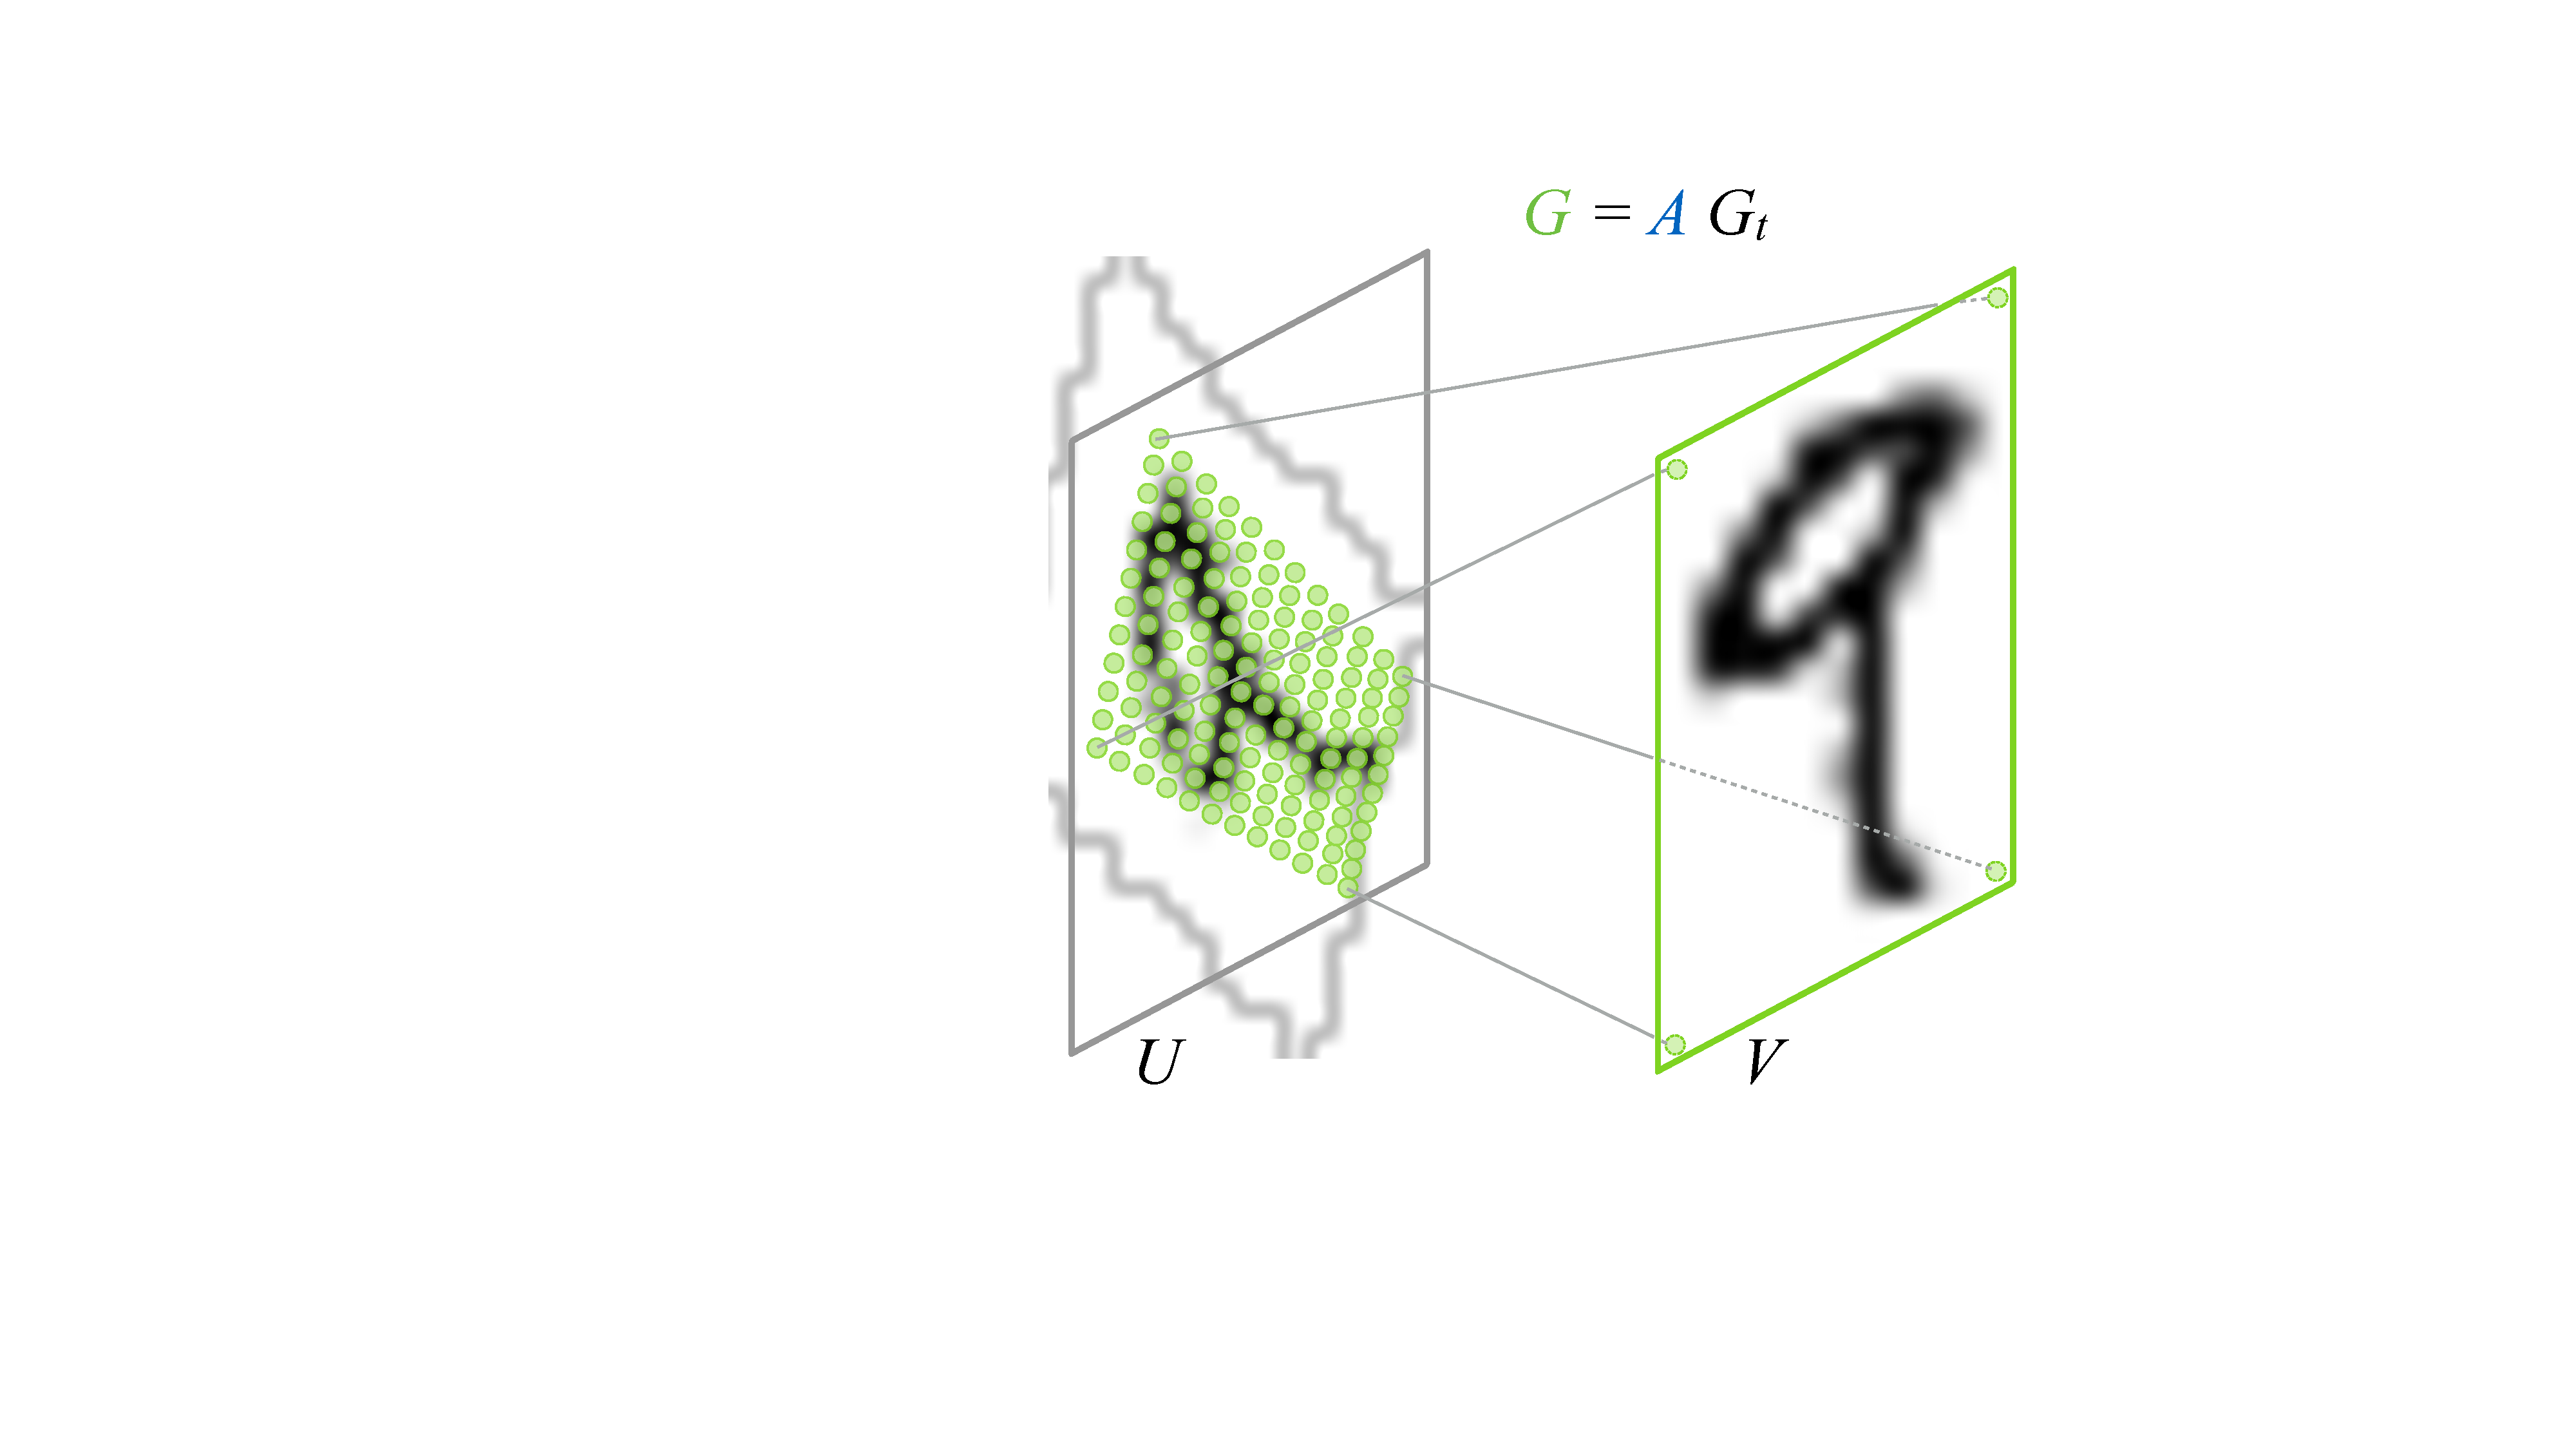
\includegraphics[width=0.35\textwidth]{trans1.pdf}
\caption{\label{fig:sample}Example sample}
\end{wrapfigure}
$$ i' = i+F[i,j,0], \; j' = j+F[i,j,1]$$
$$ V[i,j] = 
(i'-\left\lfloor{i'}\right\rfloor)U[\left\lfloor{i'}\right\rfloor,j] + (\left\lceil{i'}\right\rceil-i')U[\left\lceil{i'}\right\rceil,j] + $$
$$ \qquad \; \; (j'-\left\lfloor{j'}\right\rfloor)U[i,\left\lfloor{j'}\right\rfloor] + (\left\lceil{j'}\right\rceil-j)U[i,\left\lceil{j'}\right\rceil]$$
$$ $$

The key property to note is that every pixel in $V$ is simply a linear combination of the pixels in $U$. This means that if we have a gradient for every pixel in $V$, we can compute a gradient for every pixel in $U$, and so errors can propagate through the grid sampler as if it were any other part of a neural network.


{\bf Weight sharing}

There is a quote that has had a lasting impact on me, it says something along the lines of: ``Most progress in deep learning  is driven by clever ways of sharing weights. Convolutional networks share weights across space. Recurrent networks weight share across time. Future innovations will be defined by how they share weights.'' I cannot find a record of this quote, but I believe it was said by Geoffrey Hinton while evangelizing Capsule Networks \cite{capsule}.

The reason I mention this is that weight sharing is an important tool used in neural network models for image registration and I want to write a short note about it so I can freely bring it up later. As I referenced above, convolution is one of the most basic forms of weight sharing. It is when weights are shared between connections in a layer of a neural network, meaning that any gradient update that happens to one of them happens to all of them. This idea can be generalized to the network level, whenever any weight in a network is updated, all corresponding weights in the other networks are updated in the same way. This is equivalent to having a single network that does multiple tasks, and then summing the gradient updates from each of those tasks. The case where weights are shared between only two networks is sometimes called a Siamese Network.

It makes sense to think about Siamese Networks when considering our task because we have symmetry in our inputs: both the source and target come from the same underlying distribution, so we would like to process them in similar but independent ways.

\newpage


%%%%%%%%%%	RELATED WORK	%%%%%%%%%%

\section{Related Work}

At this point, it will be assumed that the reader understands what the alignment, registration, and optical flow tasks entail. Now, I will organize the landscape of prior work with respect to the dimensions that I know are important to the work being done in Seunglab, and I believe are important to general applications of these tasks. They are the following:
\begin{enumerate}
\item {\bf Coarse-to-fine vs. One-shot.} A course-to-fine method processes the source and target at multiple levels of downsampling (multiple resolutions), while a one-shot method only processes the originals. Coarse-to-fine is a classic idea in the vision community and is desirable because it enables greater field-of-view for fewer parameters.
\item {\bf Dense vs. Parametrized. } A dense method creates its prediction by computing a vector field that it uses to sample the source, while a parametrized method computes some parametrization that is not a vector field and uses it to generate a vector field to sample the source. Dense is desirable because it can represent any deformation.
\item {\bf Weakly supervised vs. Strongly supervised.} A weakly supervised method backpropagates on its prediction but not on the transformation used to obtain it, while a strongly supervised method backpropagates on the transfomation. Weakly supervised is desirable because we will not always have the correct answer for the transformation, but we will always have the correct answer for the prediction (the target).
\item {\bf Learned vs. Fixed.} A learned method is one that is differentiable and hence can be optimized with gradient descent, a fixed method is not differentiable and hence cannot be optimized.
\end{enumerate}

With these characteristics in mind, we will be better equipped to sift through models that accomplish some subset of the goals we want to achieve. As shown below, the current system for alignment has none of the desired characteristics, we know of eight previous models that have some subset of the characteristics, and our approach will have all of them. 

\begin{center}
\begin{tabular}{l c c c c}
  	Method & Course-to-fine? & Dense? & Weakly supervised? & Learned?  \\ \hline
    {\bf Old} &            &            &            &            \\
    WarpNet \cite{warpnet}	      &            &            &            & \checkmark           \\
    ssEMnet	\cite{ssemnet}      &            &            &  \checkmark          & \checkmark           \\
    VoxelMorph \cite{voxelmorph}	  &            &  \checkmark          &  \checkmark          & \checkmark           \\
    VoxelMorph' \cite{voxelmorph_clone}  &            &  \checkmark          &  \checkmark          & \checkmark          \\
    FlowNet	\cite{flownet}      &            &  \checkmark          &            & \checkmark           \\
    UnFlow	\cite{flownet}      &            &  \checkmark          & \checkmark           & \checkmark           \\
    SpyNet \cite{spynet}	      & \checkmark           &  \checkmark          &            & \checkmark           \\
    SpyNet+	\cite{spynet_plus}      & \checkmark           &  \checkmark          &            & \checkmark           \\
    {\bf Now}  & \checkmark & \checkmark & \checkmark & \checkmark
\end{tabular}
\end{center}

\newpage

The table above captures a somewhat over-simplified view of our research problem, because there is a lot of nuance behind how each check is implemented. This being said, the line of abstraction has to be drawn somewhere, and I believe the reader is now prepared to head to the next section and learn about our approach if they want to cut to the chase. For the reader that would like to peak into the previous models in more detail and learn about the specific reasons we want to improve upon hem, I have included descriptions of prior models and their shortcomings.

{\bf Old.} The current system for alignment is called Alembic. At its core is a spring-based technique for elastic registration \cite{elastic_alignment}. For every slice in the volume, correspondences between patches in it and patches in the next slice are found using normalized cross correlation. Normalized cross-correlation is a measure of similarity that resembles convolution. Each of these correspondences is treated as a spring, where the energy stored in the spring is proportional to the square of its distance. Then, the system is iteratively minimized by letting all the patches shift around and relax their springs.

\begin{figure}[H]
\centering
\includegraphics[width=0.7\textwidth]{elastic.png}
\caption{\label{fig:elastic}An illustration of the spring-mesh from the original paper \cite{elastic_alignment}.}
\end{figure}

Above I summarized the reasons we need to replace this system, but here I will elaborate on them in more detail:
\begin{itemize} 
  \item {\bf Static.} This model is not learned in any way. The humans that invented it sat down and thought through all its details, and some humans in Seunglab sit down and babysit it through the alignment process. It is fickle and costly to manage.
  \item {\bf Constrained.} This model executes a piece-wise affine transformation on the unaligned volume to get the aligned volume. This is all it can do, so it will never be able to correct deformations that are more sophisticated than affine warping or deformations that are discontinuous, like cracks and folds, which are handled manually.
\end{itemize}

The solution to the first problem is to use a model that can be learned, i.e. a differentiable one. The solution to the second problem is to use a model that can apply more sophisticated transformations.

{\bf WarpNet.} In 2016 some researchers at the University of Maryland and NEC Labs published WarpNet \cite{warpnet}, a deep learning based technique for single-view reconstruction. The goal of single-view reconstruction is to get a conception of a 3D object from 2D images of it at different viewpoints. The core operation in their pipeline was image registration. They used a Siamese network to learn the parameters of a piece-wise affine transform and trained it based on correspondence matching within their reconstruction. Their architecture is shown in the following figure.

\begin{figure}[h!]
\centering
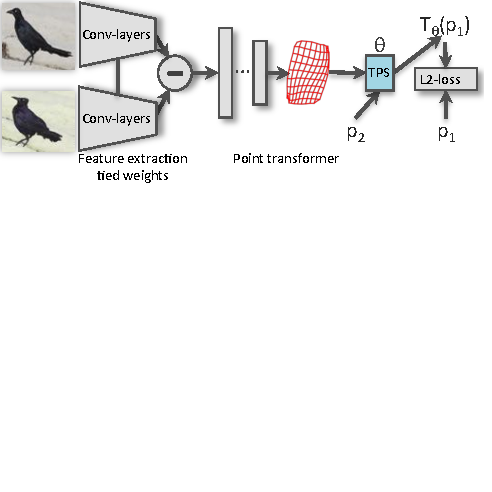
\includegraphics[width=0.7\textwidth]{warp_arch.pdf}
\caption{\label{fig:warpnet}The WarpNet architecture \cite{warpnet}.}
\end{figure}

This model is a step closer to what we need in that it is differentiable, but it is not viable because its transformation is constrained to piece-wise affine transformations.

{\bf ssEMnet.} This paper tackles the same problem Seunglab is concerned with: aligning EM images of the brain. Their approach is to take two adjacent images, stick an affine spatial transformer (like in the original paper \cite{stn}) on top of one image, encode the spatially transformed version of one image and the original version of the other image, and minimize the distance between these two encodings. They get decent looking results, but their issue is the same as WarpNet: their transform is too heavily constrained.

{\bf VoxelMorph.} This year there was a paper out of MIT presenting a deep learning technique for deformable medical image registration \cite{voxelmorph}. Their problem is extremely similar to ours; the main difference is that they are working with MRI scans of brains, not EM images of them. Their technique consisted of a U-net-like \cite{unet} architecture that takes in a source and target outputs a dense vector field describing how to transform the source to get the target. It is trained on the difference between the target and prediction and a smoothness term.

{\bf VoxelMorph'.} In 2015 there was a very similar paper \cite{voxelmorph_clone} out of the Beihang University in China. All the details mentioned about VoxelMorph apply to it as well.

{\bf FlowNet.} This work \cite{flownet} from 2015 is concerned with the more general task of learning optical flow with CNNs. They test their method on synthetic video, but it is designed to be applicable to domains such as ours. They achieve nice looking results on their data, albeit by directly supervising their field and using a massive architecture, which is pictured below.

\begin{figure}[h!]
\centering
\includegraphics[width=0.9\textwidth]{flownet_arch.png}
\caption{\label{fig:flownet}The (more complex) FlowNet architecture \cite{flownet}.}
\end{figure}

{\bf UnFlow.} This paper \cite{unflow} takes the architecture in FlowNet and presents a way to weakly supervise it. Instead of directly training on error in the field, they train on error in the predicted image, and create a scheme where they do this forward and backward through a video.

These models are decent at their task, but they seem unnecessarily large.  Historically, computer vision models have seen efficiency gains from enriching an input image by turning it into an image pyramid. That is, instead of processing the images as they are, they could be processed many times at different scales (starting from coarsest and moving to finest).

{\bf SpyNet.} The spatial pyramid transformer network paper \cite{spynet} made the idea of coarse-to-fine optical flow happen. In this model, a source and target are taken as input and then processed at multiple levels. Each level computes a residual field that contributes to the end field. The higher-level / lower-resolution residuals are computed first and then applied to the source images below them, so each level only has a small job to do. The model is trained with direct supervision on the residuals at every level, and achieves performance comparable to FlowNet with (1/30)th of the parameters. 

{\bf SpyNet+.} A paper \cite{spynet_plus} put on Arxiv about a month ago extends SpyNet by making the network at each level more complex. It is unclear if this is beneficial to the network or not, as this paper applies the architecture a different task: remote sensing in aerial images. 

\begin{figure}[h!]
\centering
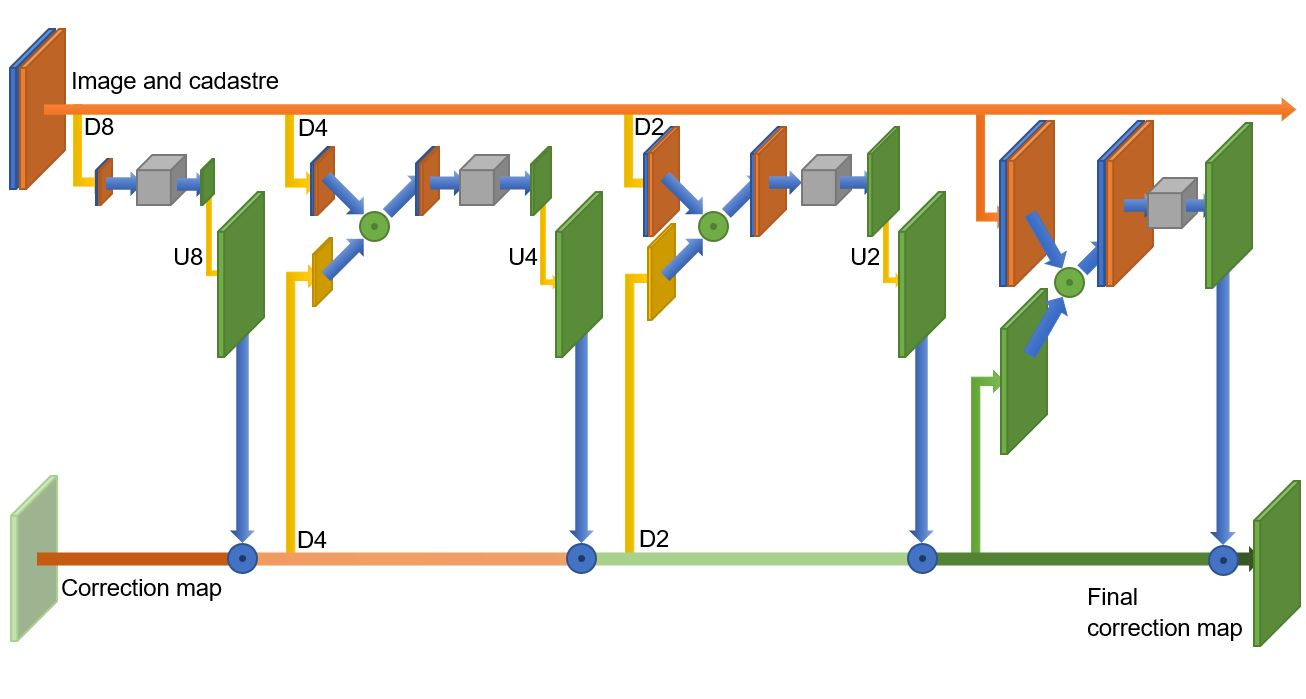
\includegraphics[width=0.9\textwidth]{py_net.jpg}
\caption{\label{fig:pynet}The general form of the Pyramid architecture \cite{spynet_plus}.}
\end{figure}

\newpage


%%%%%%%%%%	APPROACH	%%%%%%%%%%

\section{Approach}

The novelty of our approach is: we take the pyramidal structure of SpyNet \cite{spynet}, but (1) allow it to operate on learned feature maps and (2) manage to train it in a weakly supervised way. This is valuable because our model can better learn more general classes of optical flow: (1) gives the network more representational power to recognize complex transformations and (2) enables the network to learn from transformations for which there is no ground-truth. A concrete manifestation of this value-add in our lab is that cracks and folds in EM images can now be mended automatically.

I will organize my description of our method into two groups and four categories: the architecture and objective, and the data augmentation and training details. Decisions about the first two were motivated by what we thought we knew theoretically and decisions about the second were motivated by what we saw happening empirically.

\subsection{Architecture}

At the top level, our network implements the optical flow specification:

\indent in: {\tt source} $(W, W)$, {\tt target} $(W, W)$

out: {\tt pred} $(W, W)$, {\tt field} $(W, W, 2)$

It does this by splitting up the problem into more manageable versions, one for each level of downsampling. At each level $i$, function $G_i$ implements:

\indent in: {\tt source\_fmaps} $(c, w, w)$, {\tt target\_fmaps} $(c, w, w)$

out: {\tt residual} $(w, w, 2)$

Note that the width of each set of matrices is $w$, the width of our matrices at that level of downsampling, as opposed to $W$, the original width. At level $i$, $w = W / 2^i$. Here is an illustration of the inputs and outputs of a few $G$'s. 

\begin{figure}[H]%
    \centering{{\includegraphics[width=\textwidth]{my_pyramid.png} }}%
    \caption{Inputs and outputs of subtasks}%
    \label{fig:example}%
\end{figure}

This diagram is only meant to illustrate the way the subproblems sit relative to each other, it is not a complete picture of our model. Our model has a lot of processing going on at each level, which I will describe now by focusing on what it looks like from the viewpoint of a single level. 

Take a look at the following diagram.

\begin{figure}[H]%
    \centering{{\includegraphics[width=\textwidth]{my_level.png} }}%
    \caption{Processing that happens at level $i$}%
    \label{fig:example}%
\end{figure}

Allow me to explain what each function is doing.\begin{itemize}
\item $s \quad$ grid-sample (as described in the background section) $\texttt{source}_i$ according to the grid $\texttt{residual}^{up}_i$. We do this because we do not want to have to redo the work we did at higher levels; we want to start from there and try to compute an even more fine grained field.
\item $u \quad$ up-sample $\texttt{residual}_i$ by a factor of 2 to get $\texttt{residual}^{up}_i$. We do this to be able to apply the information in $\texttt{residual}_i$ on the level below. 
\item $D_i \quad$ generate the $(i+1)th$ set of features for $\texttt{source}_i$ / $\texttt{target}_i$. This function is like a smart downsampler. It's specification is:

\indent in: {\tt curr\_fmaps} $(c, w, w) \qquad$ out: {\tt next\_fmaps} $(c, \frac{1}{2}w, \frac{1}{2}w)$

Note that this is a single network performing two runs at every iteration, a.k.a. a Siamese network.
\item $S_i \quad$ interpret the features for $\texttt{source}_i$ / $\texttt{target}_i$ into a shared representational format. The motivation for doing this is that there might be some common way of unpacking the feature maps into a hidden layer, like in RNNs for language. If there are $h$ channels in the representation, this function's specification is

\indent in: {\tt fmaps} $(c, w, w) \qquad$ out: {\tt rep} $(h, w, w)$

Note again that this is a single Siamese network.
\item $J_i \quad$ process the concatenated representations for $\texttt{source}_i$ and $\texttt{target}_i$ into $\texttt{residual}_i$. This function's specification is

\indent in: {\tt reps} $(2h, w, w) \qquad$ out: {\tt residual} $(w, w, 2)$
\end{itemize}

Note the following corner cases. On the bottom level, the input feature maps (the ones from ``below'') are simply the original source and target. On the top level, the input residual (the one from `` above'') is the identity grid.

Lastly, let me tie up the loose ends about how these residuals are used. The residual at level $i$ is up-sampled $i$ times by a factor of $2$ to get a field of dimension $(W, W, 2)$. All of these fields are added to produce the output field, and the source is sampled with this field to get the prediction.

This concludes my general specification of our architecture. As a concrete example, I will describe the settings of the components above that yield good results in our domain. We use 5 levels, with base images of size $1024 \times 1024$. There are four feature maps at each level for the source/target, but one is reserved for a downsampled version of the original source/target. We implement $D_i$, $S_i$, and $J_i$ as CNNs with 2D same convolutional layers, kernels of size 5, and ReLU activation. $D_i$ has 2 convolutional layers with 3 output channels each, followed by an average pool. $S_i$ has 2 convolutional layers, the first having 32 output channels and the second having 64. $J_i$ has 3 convolutional layers, the first having 64 output channels, the second having 32, and the third having 2.

\subsection{Objective}

The learning objective dictates what we want our model to prioritize. It is the most finicky and fine-tuned component of our approach. Our loss function is a weighted sum between a term for the similarity between the target and prediction, and a term for the smoothness of the field used to obtain the prediction.
$$ \mathcal{L}(S, T, F) = d(S, T) + \lambda \; s(F)$$

The functions $d$ and $s$ that we use are relatively simple; we tested more complex ones but they did not seem to make a noticeable difference.

Define $\mathcal{V}$ as the set of pixel positions $[i,j]$ where $S[i,j] \neq 0$ and $T[i,j] \neq 0$. This is the set of positions where both the source and target are valid.

$$ d(S,T) = \cfrac{1}{|\mathcal{V}|} \sum\limits_{(i, j) \in \mathcal{V}} \Big( S[i,j] - T[i,j] \Big)^2 $$

Our distance metric is the mean squared error over (MSE) all the valid pixel pairs in the source and target. The reason we use this instead of MSE is the following problematic occurrence. Say there are two slices, one above the other, that were originally aligned, but then one of them lost a strip off its end. The part that remains is still aligned with its corresponding part in the other slice, so a deformation fixer should not touch these slices. But we found that networks trained on normal MSE try to stretch out the slice with a strip taken out to compensate, since the MSE in the missing section was so severe. MSE over non-zero pixel pairs does not have this problem, and still learns from the sections that are present.

Let $w$ be the side length of $S$, $T$, and $F$. Define $\mathcal{N}_{ij}$ as the set of neighbors of pixel position $(i',j')$ that satisfy $0 \leq i' < w$ and $0 \leq j' < w$ .
$$ s(F) = \cfrac{1}{w^2} \sum\limits_{i=0}^{w-1} \sum\limits_{j=0}^{w-1} \sum\limits_{(i', j') \in \mathcal{N}_{ij}} \left\| F[i,j] - F[i',j'] \right\| ^2 $$

Our smoothness metric is the squared differences between neighboring vectors in the output field. Although there are functions that are more theoretically appealing, like those describing elastic compression, they could not outperform our first instinct, this function, so we stuck with it. 

\subsection{Augmentation}

An important component of our approach is the extensive data augmentation we do to train the network. We parametrize difficult deformations and situations and apply random instances of our synthetic versions of them to our data at training time. The hope that this will better expose the network to their true underlying distribution. I will describe them in approximate order of complexity, but before I begin, let me show what all of the transformations look like when applied together.

\begin{figure}[ht]%
    \centering
    \subfloat[Original]{{\includegraphics[width=0.40\textwidth]{original_source.png} }}%
	\qquad
    \subfloat[Deformed]{{\includegraphics[width=0.40\textwidth]{new_source.png} }}%
    \caption{All types of data deformations composed together}%    \label{fig:example}%
\end{figure}

{\bf Chop.} For a randomly selected side of the image and a randomly selected distance $d$, set all pixels that are at most $d$ away from that side to $0$. This zeros out a strip on one side of the image.

{\bf Pad.} Add a border of zeros all around both the source and the target. Note that this is not zeroing out existing pixels, it is adding to the width.

{\bf Sync-rotate.} Rotate both the image and its partner (both the source and target) by $90^{\circ}$ a random number of times.  

{\bf Translate.} Translate the image by a randomly selected distance $d$. New pixels are all black.

{\bf Free-rotate.} Rotate the image by a randomly selected angle $\theta$. 

{\bf Affine-warp.} Sample the image according to the noisy identity grid 
\[
\begin{bmatrix}
    1 + \epsilon_{xx}		& \epsilon_{xy}  		& \epsilon_{x} \\
    \epsilon_{yx}       	& 1 + \epsilon_{yy}  	& \epsilon_{y} \\
\end{bmatrix}
\]

{\bf Tone.} Select a square patch at a random position with a random width. Either tone it down by halving its values, or tone it up by halving the distance between each of its values and 1 (maximum brightness).

{\bf Crack.} This is the most involved transformation, since it is highly specialized to our domain. First, the crooked line in the middle of a crack is defined with a random walk. This random walk starts on a randomly chosen side of the image and then proceeds by repeatedly making one of three choices: forward, right, or left, until it hits another side of the image. The probabilities of each of these directions can be anything, but the most realistic results are achieved when they differ, so the crack has a tilt. Once the line has been decided, the two pieces are moved. Each moves a distance $d$ at angle $\theta$, both of which are randomly drawn. Since we want the pieces to move in opposite directions, these distributions are opposites.

\newpage


%%%%%%%%%%	IMPLEMENTATION	%%%%%%%%%%

\section{Implementation}

I think it would be a waste of space to run through a play-by-play of every module I wrote while working on this project. My code can be found at \href{github.com/skeselj}{github.com/skeselj} and Eric's code at \href{github.com/emitch}{github.com/emitch}. Instead, I would like to briefly discuss non-obvious implementation details about two key processes: how the model is initialized and how it is trained.

\subsection{Initialization}

The fields used to sample images are represented using the coordinate range $[-1, +1]$ ($-1$ is left/bottom, $+1$ is right/top). Since our network is deep and uses ReLU activation, there is a reasonable chance some vectors in its initial output fields will be outside this range, or at least far from their corresponding vectors in the identity grid. This would be problematic because the information we need to make updates is local, and scattered vectors could make the initial gradients large and noisy. These in turn might take the model far away from its near-optimal area, where it might get stuck in a local minimum and never reach a reasonable answer. Since the problem we face is that the initial fields are not enough like the identity grid, a reasonable course of action is to make the initial fields more like the identity grid. A natural way to do this is to downscale the weights and biases of the last layer. This will make the initial residuals close to zero, so the network has access to local information, but not actually zero, so the network can make non-miniscule updates. The specific downscaling value I use is 100, but Eric uses 10 and his networks work.

All neural network frameworks I know of implement some form of Xavier initialization, which randomly draws weights from uniform distributions such that their expected sum is zero and the expected variance of each layer is 1. Or rather, they implement something like Xavier initialization. In working on this project, Eric discovered that PyTorch actually has the Xavier initialization formula slightly off from what it theoretically should be. A layer of $k \times k$ kernels with $n$ input channels will have expected standard deviation ${1} / {\sqrt{nk^n}}$. The uniform distribution on $[A, B]$ has standard deviation $\sqrt{{(B-A)^2} / {12}}$. To preserve the standard deviation and make the weights sum to zero in expectation, the weights should be drawn from $U(-\sigma, +\sigma)$, with $\sigma = \sqrt{ {3} / nk^n }$. However, in the PyTorch code they are drawn with $\sigma = \sqrt{ {1} / nk^n }$. Eric filed a bug report on the PyTorch project girhub and one of the main curators of PyTorch replied to it, saying this is the result of a historic bug that appears to have empirically worked better (you can see the bug thread here: \href{https://github.com/pytorch/pytorch/issues/6950}{https://github.com/pytorch/pytorch/issues/6950}). Evidently, the bug seems to not be much of an issue for many PyTorch users, or else they would have raised this issue before. Since I have seen no empirical evidence that theoretically incorrect way works better on our task, I have used the theoretically correct way ever since Eric discovered it. To be fair, I have no empirical evidence that the theoretically correct way works better either, but at least it is theoretically correct.

\subsection{Training}

The data used to generate the results in this paper is stored as 100 stacks. Each stack has 50 slices and each slice is 1024 x 1024 pixels. A single stack is run through the model by first running all its pairs in one direction (top to bottom), and then all its pairs in the other direction (bottom to top). This would yield 98 pairs, which is annoying, so the first pair in each direction is run again to make 100 pairs per stack. Intuitively, I think it is helpful to train the model stack by stack, because this gives some sort of local regularity to the model's learning. A few weeks ago I was training models by pulling random pairs from a single, huge stack, and was struggling to get nice results. To be fair, the architecture was slightly different, so it is unclear if the stack organization mattered.

Since there are 100 stacks of 100 pairs in my training data, there are 10,000 pairs per training trial. On an NVIDIA GeForce GTX 1080 Ti GPU, an entire training trial takes about 3 hours, i.e. a single pair takes about 1 second. A speedup trick that has helped is staging the training of the levels. By this I mean that first the top levels are trained, with the lower levels fixed at the identity grid, and then gradually the lower levels are allowed to participate. This saves time because in the early iterations only the top levels are doing computation. The specific schedule is to only train the top layer on the first 10 stacks, then the top and second from the top on the next 10, and so forth up until all layers are getting trained for stacks 40-100.


\newpage


%%%	RESULTS

\section{Results}

Now the fun part: let me show you what this thing can do. I will organize my exploration into three parts. First, I will show what the model outputs for different types of inputs. Then, I will take a look at the inner workings of the model. Finally, I will compare the results our model achieves to those achieved by a model that much larger in size but lacks our model's defining structural characteristics.

\subsection{Eye test}

Each of the following pages contains a set of six images: source, target, prediction, original distance, new distance, and field. I will refer to this set of images as a snapshot. The source, target, prediction, and field refer to the entities by the same names described above. The original distance is the pixel-wise absolute value of the image you get when you subtract the source from the target, and the new distance is the pixel-wise absolute value of the image you get when you subtract the prediction from the target. All the image plots represent 0 with black and 1 with white. The field image is a vector plot, where each vector's length is its true length and each vector's color is determined by its direction. The color map is a rainbow with red meaning directly to the right.

\newpage

\begin{figure}[H]
\centering
\subfloat[source]{
  \includegraphics[width=0.42\textwidth]{trans_source.png}
}
\hspace{3mm}
\subfloat[target]{
  \includegraphics[width=0.42\textwidth]{trans_target.png}
}
\hspace{0mm}
\subfloat[original distance]{
  \includegraphics[width=0.42\textwidth]{trans_ogdiff.png}
}
\hspace{3mm}
\subfloat[prediction]{
  \includegraphics[width=0.42\textwidth]{trans_pred.png}
}
\hspace{0mm}
\subfloat[new distance]{   
  \includegraphics[width=0.42\textwidth]{trans_mydiff.png}
}
\hspace{3mm}
\subfloat[field]{
  \includegraphics[width=0.42\textwidth]{trans_field.png}
}
\caption{Translation snapshot}
\end{figure}

\newpage

\begin{figure}[H]
\centering
\subfloat[source]{
  \includegraphics[width=0.42\textwidth]{rot_source.png}
}
\hspace{3mm}
\subfloat[target]{
  \includegraphics[width=0.42\textwidth]{rot_target.png}
}
\hspace{0mm}
\subfloat[original distance]{
  \includegraphics[width=0.42\textwidth]{rot_ogdiff.png}
}
\hspace{3mm}
\subfloat[prediction]{
  \includegraphics[width=0.42\textwidth]{rot_pred.png}
}
\hspace{0mm}
\subfloat[new distance]{   
  \includegraphics[width=0.42\textwidth]{rot_mydiff.png}
}
\hspace{3mm}
\subfloat[field]{
  \includegraphics[width=0.42\textwidth]{rot_field.png}
}
\caption{Rotation snapshot}
\end{figure}

\newpage

\begin{figure}[H]
\centering
\subfloat[source]{
  \includegraphics[width=0.42\textwidth]{affine_source.png}
}
\hspace{3mm}
\subfloat[target]{
  \includegraphics[width=0.42\textwidth]{affine_target.png}
}
\hspace{0mm}
\subfloat[original distance]{
  \includegraphics[width=0.42\textwidth]{affine_ogdiff.png}
}
\hspace{3mm}
\subfloat[prediction]{
  \includegraphics[width=0.42\textwidth]{affine_pred.png}
}
\hspace{0mm}
\subfloat[new distance]{   
  \includegraphics[width=0.42\textwidth]{affine_mydiff.png}
}
\hspace{3mm}
\subfloat[field]{
  \includegraphics[width=0.42\textwidth]{affine_field.png}
}
\caption{Affine warp snapshot}
\end{figure}

\newpage

\begin{figure}[H]
\centering
\subfloat[source]{
  \includegraphics[width=0.42\textwidth]{crack_source.png}
}
\hspace{3mm}
\subfloat[target]{
  \includegraphics[width=0.42\textwidth]{crack_target.png}
}
\hspace{0mm}
\subfloat[original distance]{
  \includegraphics[width=0.42\textwidth]{crack_ogdiff.png}
}
\hspace{3mm}
\subfloat[prediction]{
  \includegraphics[width=0.42\textwidth]{crack_pred.png}
}
\hspace{0mm}
\subfloat[new distance]{   
  \includegraphics[width=0.42\textwidth]{crack_mydiff.png}
}
\hspace{3mm}
\subfloat[field]{
  \includegraphics[width=0.42\textwidth]{crack_field.png}
}
\caption{Crack snapshot}
\end{figure}

\newpage

\begin{figure}[H]
\centering
\subfloat[source]{
  \includegraphics[width=0.42\textwidth]{all_source.png}
}
\hspace{3mm}
\subfloat[target]{
  \includegraphics[width=0.42\textwidth]{all_target.png}
}
\hspace{0mm}
\subfloat[original distance]{
  \includegraphics[width=0.42\textwidth]{all_ogdiff.png}
}
\hspace{3mm}
\subfloat[prediction]{
  \includegraphics[width=0.42\textwidth]{all_pred.png}
}
\hspace{0mm}
\subfloat[new distance]{   
  \includegraphics[width=0.42\textwidth]{all_mydiff.png}
}
\hspace{3mm}
\subfloat[field]{
  \includegraphics[width=0.42\textwidth]{all_field.png}
}
\caption{All transformations snapshot}
\end{figure}

\newpage

I am proud of what these samples look like, and they are not cherry-picked! Each set of samples was generated in the following way. A fresh model was trained on 100 unaligned, randomly augmented stacks, i.e. 10,000 pairs. The snapshot for the last pair in each stack was saved. The samples above are either the last or second last saved snapshot (sometimes the last one was not representative of the transformation being investigated). 

Allow me to discuss what I think are the most notable observations about what we see above, some good and some perhaps not.

{\bf Field and prediction sanity.} In the cases where we have a good conception of what the field should be (translation, rotation, and crack) the network outputs a field that resembles what we know is correct. In the more general case, we know the fields should be smooth, because both synthetic and real deformations are smooth, and the fields are generally smooth. For the prediction we always have a good conception of what we approximately want: the target. In all the samples above, even the really deformed last one, the prediction resembles the target.

{\bf Distance reduction and patchiness. } For a more detailed view of how closely the prediction resembles the target, we can consult the new distance images, especially as they relate to the original distance images. Across all samples, the distance seems to decrease drastically after we apply our field to the source. I am not sure how to feel about this. While it is true that we want the prediction to look like the target, we do not want the two to be identical because then the information in the source would be destroyed. Our motivation for sampling the source to get the prediction was to conserve this information, but it seems our network is finding clever ways to alter the source tissue. To see an example of this, look at the source and prediction of the last snapshot, and notice how the black patches lighten after we apply the complicated field. In this case the dark patches were deformations that we put there ourselves, so we would want the model to get rid of them, but what if the network is destroying structure we are interested in?

This question has been a perennial worry throughout the course of this project. We can sit and eye-ball the ways these different pairs of images resemble each other, but our human eyes can only gauge large-scale deformations. The most reliable way of seeing if this model is destroying information we are interested in would be to stick our model into the connectomics pipeline and see if the results improve or degrade. This is on the horizon, but we have not done it yet. The step before that is to peak at the z-axis of stacks aligned using our model to see if anything is going awry. An example of one such stack is shown below. It looks pretty nice, blood vessels (big white blobs) and mitochondria (small black blobs) are smoothly visible. The horizontal black lines we see correspond to dark or empty slices; it is reassuring that they do not throw off the alignment.

\vspace{0.5cm}

\begin{figure}[h!]
\centering
\includegraphics[width=\textwidth]{zaxis_old.png}
\caption{\label{fig:zaxis} The z-axis perspective of an aligned stack.}
\end{figure}

\subsection{Under the hood}

To properly understand how our model is behaving, it seems necessary to analyze not only its outputs, but also the way it operates to produce these outputs. In this subsection I will explore: the errors our model makes as it trains, the residuals it uses to calculate the output field, and the feature maps it builds to represent its inputs. My aim is to get a better sense for how our model operates and evaluate the usefulness of our design choices. 

{\bf Errors}

The following are the training curves for mean squared error (MSE) and smoothness loss (SMO) for a trial using the combined augmentations. 

\vspace{0.5cm}

\begin{figure}[ht]%
    \centering
    \subfloat[MSE]{{\includegraphics[width=0.45\textwidth]{training_plot_mse.png} }}%
	\qquad
    \subfloat[SMO]{{\includegraphics[width=0.45\textwidth]{training_plot_smo.png} }}%
    \caption{Training curves for the two components to our loss}%    \label{fig:example}%
\end{figure}

At first glance these plots might seem uninteresting, but they offer useful leads about what aspects of our model we should investigate. The most salient features are the sharp spikes, reflecting a few catastrophic mistakes. Even though these are extremely rare (about 10/100,000) they have the capacity to completely mess up an alignment, because every slice depends on every slice before it. It would be nice to get an idea of what types of samples cause these catastrophic mistakes. Although I did not monitor for particularly bad samples when generating the training curves above, I retrained the model on 10 lightly augmented stacks and recorded the (source, target) pair that produced the highest error. It is shown below.

\begin{figure}[ht]%
    \centering
    \subfloat[Source]{{\includegraphics[width=0.45\textwidth]{worst_source.png} }}%
	\qquad
    \subfloat[Target]{{\includegraphics[width=0.45\textwidth]{worst_target.png} }} \\
     \subfloat[Prediction]{{\includegraphics[width=0.45\textwidth]{worst_pred.png} }}%
	\qquad
    \subfloat[New distance]{{\includegraphics[width=0.45\textwidth]{worst_mydiff.png} }}%
    \caption{A problematic sample}%    \label{fig:example}%
\end{figure}

Looking at these examples, it is understandable that the error of the model's prediction on them is so great. With such a bright source that is sparse with information, anything the model does will drastically disagree with the target. Although this realization does not make the error any less of an error, it is valuable in that it informs us what we need to look out for.

Returning to our analysis driven by details in the training curves, there is another feature displayed in them that I would like to highlight: the interaction between mean squared error and smoothness loss. At face-value, we see that MSE grossly dominates SMO; it is over 1,000 bigger. This raises the question: is SMO loss doing anything useful? If no, we should get rid of it. If yes, perhaps we should amplify its coefficient. The answer to this question is yes, but it should not be amplified because you can have too much of a good thing. When I searched over smoothness term coefficients I found that $\lambda =$ 5,000 yielded the best looking results, below I have shown what three different settings of the smoothness coefficient cause a model to do on the same cracked sample.

\begin{figure}[ht]%
    \centering
    \subfloat[$\lambda =$ 50]{{\includegraphics[width=0.28\textwidth]{field_patchy.png} }}%
	\qquad
    \subfloat[$\lambda =$ 5,000]{{\includegraphics[width=0.28\textwidth]{field_justright.png} }}%
    \qquad
    \subfloat[$\lambda =$ 500,000]{{\includegraphics[width=0.28\textwidth]{field_smooth.png} }}%
    \caption{Fields produced on the same sample, for different smoothness term coefficients}%    \label{fig:example}%
\end{figure}

It seems the SMO term is acting as a useful constraint even though it is so much smaller than MSE. Indeed, if you look closely at the training curves, you can see that there is a downward trend in the MSE plot and an upward trend in the SMO plot. It is remarkable to me that two terms that differ in magnitude so greatly appear to be linked. I believe what is causing this is high variance but low expectation in the MSE gradient, and low variance and low expectation in the SMO gradient. That is, MSE is making a lot more commotion than SMO, but they are both guiding the gradient similarly. I will admit that this theoretical musing is a bit of a reach. Regardless of the underlying machination, the bottom line is that when the smoothness coefficient is significantly lower than 5,000 we see too much patchiness, and when it is significantly higher we see fine objects like cracks ignored.


{\bf Residuals}

The explicit errors in our output image and field are nice to have because they are hard numbers, but they sit at the top level of abstraction of our complex and opaque model. Even though I cannot produce quantitative measures for the usefulness of the parts of the model leading up to the output, it would still be insightful to peak at what these components look like. A natural set of components to start looking at are the residuals that come together to form the field. Below I have visualized the five residuals that came together to form the field in Figure 15 above, the snapshot of all the transformations composed together. 

\newpage

\begin{figure}[H]
\centering

\hspace{0mm}
\subfloat[5th (top) residual]{   
  \includegraphics[width=0.42\textwidth]{res4.png}
}
\hspace{0mm}
\subfloat[4th residual]{
  \includegraphics[width=0.42\textwidth]{res3.png}
}
\hspace{0mm}
\subfloat[3rd residual]{
  \includegraphics[width=0.42\textwidth]{res2.png}
}
\hspace{0mm}
\subfloat[2nd residual]{
  \includegraphics[width=0.42\textwidth]{res1.png}
}
\hspace{0mm}
\subfloat[1st (bottom) residual]{
  \includegraphics[width=0.42\textwidth]{res0.png}
}
\hspace{0mm}
\subfloat[field (sum of residuals)]{
  \includegraphics[width=0.42\textwidth]{resfield.png}
}
\caption{Residuals and final field on the all transformations sample above}
\end{figure}

It is difficult to confidently interpret what we see above. Every layer is certainly doing something. This seems to be a point in favor of using a pyramid of residuals, because if an individual layer could easily learn all that needs to be learned, it probably would. The fact that the bottom layers are still contributing implies that they can do something the upper levels cannot that helps reduce the error. However, whether this thing they are doing is truly useful is up for debate. The lower layers are distastfully patchy, and could be performing local optimizations around individual cell bodies. We do not want to over-optimize on this level because it might destroy small-scale detail and induce jitter. On the other hand, with artifacts like cracks we have to have small-scale capabilities because their edges are always on a small-scale. It is a difficult tradeoff that it seems the current model setting adequately balances, but could always be balanced better. 

{\bf Feature Maps}

In similar spirit to our investigation of the residual maps, let us look at the feature maps that the model is using to compute each residual. Remember the setup: for the source/target, at every layer there is a downsampled version of the source/target and three learned maps. The feature pyramid for the source and target are generated using the same kernels and do not mix when being generated. The images below illustrate these maps for a single (source, target) pair after a full training trial. I normalized each map by its maximum value and sorted the maps in order of brightness. 


\newpage


\begin{figure}[H]
\begin{tabular}{cccc}
\subfloat[original 1]{\includegraphics[width = 1.2in]{src_fmap_0_0}} &
\subfloat[map 1-1]{\includegraphics[width = 1.2in]{src_fmap_0_3}} &
\subfloat[map 1-2]{\includegraphics[width = 1.2in]{src_fmap_0_2}} &
\subfloat[map 1-3]{\includegraphics[width = 1.2in]{src_fmap_0_1}}\\
\subfloat[original 2]{\includegraphics[width = 1.2in]{src_fmap_1_0}} &
\subfloat[map 2-1]{\includegraphics[width = 1.2in]{src_fmap_1_1}} &
\subfloat[map 2-2]{\includegraphics[width = 1.2in]{src_fmap_1_3}} &
\subfloat[map 2-3]{\includegraphics[width = 1.2in]{src_fmap_1_2}}\\
\subfloat[original 3]{\includegraphics[width = 1.2in]{src_fmap_2_0}} &
\subfloat[map 3-1]{\includegraphics[width = 1.2in]{src_fmap_2_1}} &
\subfloat[map 3-2]{\includegraphics[width = 1.2in]{src_fmap_2_2}} &
\subfloat[map 3-3]{\includegraphics[width = 1.2in]{src_fmap_2_3}}\\
\subfloat[original 4]{\includegraphics[width = 1.2in]{src_fmap_3_0}} &
\subfloat[map 4-1]{\includegraphics[width = 1.2in]{src_fmap_3_3}} &
\subfloat[map 4-2]{\includegraphics[width = 1.2in]{src_fmap_3_2}} &
\subfloat[map 4-3]{\includegraphics[width = 1.2in]{src_fmap_3_1}}\\
\subfloat[original 5]{\includegraphics[width = 1.2in]{src_fmap_4_0}} &
\subfloat[map 5-1]{\includegraphics[width = 1.2in]{src_fmap_4_2}} &
\subfloat[map 5-2]{\includegraphics[width = 1.2in]{src_fmap_4_1}} &
\subfloat[map 5-3]{\includegraphics[width = 1.2in]{src_fmap_4_3}}\\
\end{tabular}
\caption{Source feature maps (bottom row is highest level)}
\end{figure}

\newpage

\begin{figure}[H]
\begin{tabular}{cccc}
\subfloat[original 1]{\includegraphics[width = 1.2in]{tgt_fmap_0_0}} &
\subfloat[map 1-1]{\includegraphics[width = 1.2in]{tgt_fmap_0_3}} &
\subfloat[map 1-2]{\includegraphics[width = 1.2in]{tgt_fmap_0_2}} &
\subfloat[map 1-3]{\includegraphics[width = 1.2in]{tgt_fmap_0_1}}\\
\subfloat[original 2]{\includegraphics[width = 1.2in]{tgt_fmap_1_0}} &
\subfloat[map 2-1]{\includegraphics[width = 1.2in]{tgt_fmap_1_1}} &
\subfloat[map 2-2]{\includegraphics[width = 1.2in]{tgt_fmap_1_3}} &
\subfloat[map 2-3]{\includegraphics[width = 1.2in]{tgt_fmap_1_2}}\\
\subfloat[original 3]{\includegraphics[width = 1.2in]{tgt_fmap_2_0}} &
\subfloat[map 3-1]{\includegraphics[width = 1.2in]{tgt_fmap_2_1}} &
\subfloat[map 3-2]{\includegraphics[width = 1.2in]{tgt_fmap_2_2}} &
\subfloat[map 3-3]{\includegraphics[width = 1.2in]{tgt_fmap_2_3}}\\
\subfloat[original 4]{\includegraphics[width = 1.2in]{tgt_fmap_3_0}} &
\subfloat[map 4-1]{\includegraphics[width = 1.2in]{tgt_fmap_3_3}} &
\subfloat[map 4-2]{\includegraphics[width = 1.2in]{tgt_fmap_3_2}} &
\subfloat[map 4-3]{\includegraphics[width = 1.2in]{tgt_fmap_3_1}}\\
\subfloat[original 5]{\includegraphics[width = 1.2in]{tgt_fmap_4_0}} &
\subfloat[map 5-1]{\includegraphics[width = 1.2in]{tgt_fmap_4_2}} &
\subfloat[map 5-2]{\includegraphics[width = 1.2in]{tgt_fmap_4_1}} &
\subfloat[map 5-3]{\includegraphics[width = 1.2in]{tgt_fmap_4_3}}\\
\end{tabular}
\caption{Target feature maps (bottom row is highest level)}
\end{figure}

\newpage

As with the residuals, it is difficult to confidently judge the innards of our network. It is certainly evident that the feature maps differ amongst each other, which is encouraging, because maps that look just like each other are redundant. It is also interesting that the top level images contain formations that are starkly different from those that appear in the actual image: map 5-1 is aggressively blurred, map 5-2 is paying special attention to the top side (perhaps that is where tissue was chopped off, or translated from) and map 5-3 is even more focused on a few bright spots. All in all, these look like feature maps that are busy doing some useful work for our model.

\subsection{Head-to-head}

We have explored many facets of our model's operation and they look encouraging, but to properly evaluate our model we must compare it to an alternative. In this section I will make one such comparison. The alternative model I will use is a version of U-net \cite{unet}, because it has had success on image-to-image tasks. The original U-net, and the U-net variant that achieved superhuman accuracy on SNEMI3D \cite{snemi} had mainly $3 \times 3$ kernels and 4 levels of downsampling. The U-net I will use has $5 \times 5$ kernels and 5 levels of downsampling. It has about 35M parameters, versus the 3M parameters of our model. I am giving it so much more representational power in an attempt to even the playing field between the two models, because I have less time to optimize the U-net. I ran both models on the same set of deformed images and took a snapshot of what each one did on the last sample, shown below.

\newpage

\begin{figure}[H]
\centering
\subfloat[source]{
  \includegraphics[width=0.42\textwidth]{us_source.png}
}
\hspace{3mm}
\subfloat[target]{
  \includegraphics[width=0.42\textwidth]{us_target.png}
}
\hspace{0mm}
\subfloat[original distance]{
  \includegraphics[width=0.42\textwidth]{us_ogdiff.png}
}
\hspace{3mm}
\subfloat[prediction]{
  \includegraphics[width=0.42\textwidth]{us_pred.png}
}
\hspace{0mm}
\subfloat[new distance]{   
  \includegraphics[width=0.42\textwidth]{us_mydiff.png}
}
\hspace{3mm}
\subfloat[field]{
  \includegraphics[width=0.42\textwidth]{us_field.png}
}
\caption{Snapshot of our model on warped, cracked sample}
\end{figure}

\newpage

\begin{figure}[H]
\centering
\subfloat[source]{
  \includegraphics[width=0.42\textwidth]{unet_source.png}
}
\hspace{3mm}
\subfloat[target]{
  \includegraphics[width=0.42\textwidth]{unet_target.png}
}
\hspace{0mm}
\subfloat[original distance]{
  \includegraphics[width=0.42\textwidth]{unet_ogdiff.png}
}
\hspace{3mm}
\subfloat[prediction]{
  \includegraphics[width=0.42\textwidth]{unet_pred.png}
}
\hspace{0mm}
\subfloat[new distance]{   
  \includegraphics[width=0.42\textwidth]{unet_mydiff.png}
}
\hspace{3mm}
\subfloat[field]{
  \includegraphics[width=0.42\textwidth]{unet_field.png}
}
\caption{Snapshot of U-net on the sample above}
\end{figure}

\newpage

This sample was the 50th in a stack of slices that I deformed and saved. I stopped training of each model here because the U-net was running slowly and not making progress. Our model takes about 3 hours to do 100 stacks, while the U-net took 8 hours to do 50, so it is about 5 times slower.  This was to be expected, since the U-net has more layers and more maps per layer.

The most conspicuous difference between the two snapshots is the color of their fields: our model's field has the smooth spectral colors of a rotation and the straight stroke of a crack, while the U-net's field is pure blue with some type of emphasis at the crack and on the top. Based on how these fields look, it would seem our model is doing a better job. This intuition is further supported by the new distance image, which is smaller for our model than for U-net, and the prediction image, which is more blurry and shifted for U-net than our model. The intuition is confirmed by the average losses of the models: $\sim475$ for ours and $\sim617$ for U-net.

These deficiencies of the U-net snapshot beget the question: would better results be produced if the smoothness coefficient were increased? I tried smoothness coefficients both above and below the one used here ($\lambda = 50$) but found that lower smoothness yielded more patchiness and higher smoothness in the best case caused the crack to be ignored, and in the worst case caused the identity grid to always be returned. The same tradeoff is also present in our model, but it seems accentuated in U-net. This experiment has far from conclusively dismissed U-net as an alternative, but it does indicate that a reasonably tuned U-net with a massive parameter advantage cannot outperform our model on a realistically deformed stack.

\newpage


%%%	CONCLUSION

\section{Conclusion}

I spent most of the results section touting the strengths of the model. I feel they are clear: the model generally produces alignments that look good and seems to leverage all its parts. The most relevant information going forward is the nature of this work's limitations and how to overcome them, so I will discuss that now. Each response corresponds to the limitation with the same number.

\subsection{ Limitations}

\begin{enumerate} 
  \item Copying. A worry I brought up when discussing Figure 15 was the possibility that when aligning a source to a target, the network destroys information in the source by working too cleverly to make it resemble the target. It seems likely that this is happening on some scale, the hope is that it is too small to matter.
    \item Dependence. In Figure 18 we saw that the model cannot help but yield an incorrect output when its source is very bright or dark. We know there are at least a few of these samples in ever stack, and the catastrophic failures they cause would likely mess up an entire stack.
  \item Comparison. In the last section, I ran a basic comparison with U-net but did not glean any definitive information. We still do not have that good of an idea about how useful our defining design choices are relative to simpler, more established models.
\end{enumerate}

{\bf Next Steps}
\begin{enumerate} 
  \item Smarter smoothness. The copying phenomenon we see must be happening by way of the vector field. These clever maneuvers the network is executing are difficult to understand, but they must exist on some manifold, which means they can be analytically described. If they can be analytically described, they can be penalized with a loss function over the field, which we could incorporate into our smoothness.  
  \item Input stacks. A simple way of getting around a few problematic stacks is to allow the network to look at substacks within the overall stack. For example, instead of just looking at the source and target (two adjacent slices), the network could look at the two slices before the source, the target, and the two slices after the target. The probability that there are three very bright or dark slices in a row is much smaller than the probability that there is one.
  \item Thorough search. The solution to my inadequate comparison is simple: take the time to do a through, principled investigation of what U-net can do on this task. A grid-search over hyperparameters and data augmentations would paint a more detailed picture.\
\end{enumerate}


\newpage


%%%	REFERENCES

\bibliography{references}{}
\bibliographystyle{plain}

\end{document}
